% 物理348–352／印刷325–329；习题1–30.
\subsection*{\hyperref[sec:1]{第1章}主题的习题}
\begin{exercise}\label{ex:1}
给出一个函数序列 $f_n:[0,1]\to[0,1]$ 的例子，使 $(f_n)_\#(\mathscr L^1\restr[0,1])=\mathscr L^1\restr[0,1]$，但 $f_n\rightharpoonup\frac12$. 这些函数能否取为 $C^1$ 函数?
\end{exercise}

\begin{exercise}\label{ex:2}
$\spadesuit$ 考虑问题
\[
\max\left\{\int|x-\mathrm T(x)|^2\dd\mu:\mathrm T_\#\mu=\nu\right\}.
\]
证明，若 $\mu$ 绝对连续，则此问题有解，且最优 $\mathrm T$ 是某个凹函数的梯度.
\end{exercise}

\begin{exercise}\label{ex:3}
在二维中，对 $\mu=f\cdot\mathscr L^2$ 与 $\nu=g\cdot\mathscr L^2$，求二次费用 $c(x,y)=|x-y|^2$ 的最优运输映射，其中 $f(x)=\frac1\pi\mathbbm1_{B(0,1)}(x)$，$g(x)=\frac1{8\pi}(4-|x|^2)$.
\end{exercise}

\begin{exercise}\label{ex:4}
设 $R:\R^d\to\R^d$ 由 $R(x)=-x$ 给出. 刻画使 $R$ 成为 $\mu$ 与 $R_\#\mu$ 之间二次费用最优运输映射的概率测度 $\mu\in\mathscr P_2(\R^d)$.
\end{exercise}

\begin{exercise}\label{ex:5}
设 $S:\R^d\to\R^d$ 由 $S(x_1,x_2,\ldots,x_d)=(x_1,x_2,\ldots,-x_d)$ 给出. 证明，若 $\mu\ll\mathscr L^d$，则 $S$ 不可能是 $\mu$ 与 $S_\#\mu$ 之间二次费用的最优运输映射. 证明，若 $S$ 在上述意义下最优，则 $\mu$ 集中于形如 $\{x_d=f(x_1,x_2,\ldots,d_{d-1})\}$ 的 Lipschitz 超曲面，其中 $f\in\Lip_1(\R^{d-1})$.
\end{exercise}

\begin{exercise}\label{ex:6}
考虑多边缘问题
\[
\min\left\{\int c(x_1,\ldots,x_N)\dd\gamma:
\gamma\in\mathscr P((\R^d)^N),\ (\pi_i)_\#\gamma=\mu_i\right\},
\]
其中 $\mu_i\in\mathscr P(\R^d)$ 为给定的紧支集测度. 假设 $\gamma$ 集中于集合 $\{(x_1,\ldots,x_N)\in(\R^d)^N:x_1+\cdots+x_N=\text{常数}\}$. 证明，若费用由 $c(x_1,\ldots,x_N)=h(x_1+\cdots+x_N)$ 给出，其中 $h:\R^d\to\R$ 为凸函数，则 $\gamma$ 最优；当 $c(x_1,\ldots,x_N)=-\sum_{i\neq j}|x_i-x_j|^2$ 时，$\gamma$ 也最优.
\end{exercise}

\subsection*{\hyperref[sec:2]{第2章}主题的习题}
\begin{exercise}\label{ex:7}
考虑 $\R$ 上的两个概率测度 $\mu$ 和 $\nu$；为简单起见，假设它们无原子且具有全支集. 设 $F_\mu$ 和 $F_\nu$ 为其累积分布函数：$F_\mu(x)=\mu((-\infty,x])$，$F_\nu(x)=\nu((-\infty,x])$. 证明，以下事实等价：
\begin{enumerate}
\item $F_\mu\geq F_\nu$；
\item 存在 $\gamma\in\Pi(\mu,\nu)$，集中于 $\{(x,y):y\geq x\}$；
\item 存在 $\mathrm T:\R\to\R$，使 $\mathrm T_\#\mu=\nu$，且对每个 $x$，$\mathrm T(x)\geq x$；
\item 从 $\mu$ 到 $\nu$ 的单调递增运输 $\mathrm T$ 对每个 $x$ 都满足 $\mathrm T(x)\geq x$.
\end{enumerate}
\end{exercise}

\begin{exercise}\label{ex:8}
证明，费用 $c(x,y)=1/|x-y|$ 在 $\Pi(\mu,\mu)$ 中有最优方案 $\gamma$，且它集中于至多两个递增图像，一个在对角线上方，另一个在对角线下方. 证明，这两个图像不重叠，而且该方案确实来自一个运输映射. 该映射是否递增?
\end{exercise}

\begin{exercise}\label{ex:9}
* 在 $\mu=\mathscr L^1\restr[0,1]$ 的情形下，求从 $\mu$ 到 $\mu$、费用为 $c(x,y)=1/|x-y|$ 的最优运输映射.
\end{exercise}

\begin{exercise}\label{ex:10}
$\spadesuit$ 假设费用 $c:\R\times\R\to\R$ 属于 $C^2$，并对每个 $(x,y)\in\R\times\R$ 满足 $\frac{\partial^2}{\partial x\partial y}c(x,y)<0$. 证明一维中 $\gamma_{\mathrm{mon}}$ 的最优性. 推出，若 $\mu$ 无原子，则存在最优映射.
\end{exercise}

\begin{exercise}\label{ex:11}
设 $A$ 和 $B$ 为两个对称正定矩阵，$L_A,L_B:\R^d\to\R^d$ 是由 $L_A(x)=Ax+a$、$L_B(x)=Bx+b$ 定义的仿射函数，其中 $a,b\in\R^d$ 已给定. 取一个在旋转下不变的参考测度 $\varrho$（即对每个满足 $R\cdot R^t=\mathrm I$ 的矩阵 $R$，都有 $R_\#\varrho=\varrho$），定义 $\mu:=(L_A)_\#\varrho$，$\nu:=(L_B)_\#\varrho$. 求从 $\mu$ 到 $\nu$ 的二次费用最优运输映射.
\end{exercise}

\subsection*{\hyperref[sec:3]{第3章}主题的习题}
\begin{exercise}\label{ex:12}
考虑区域 $\Omega=[0,3]\times[0,2]$ 及其上的两个绝对连续测度 $\mu_0$ 与 $\mu_1$，密度分别为 $\varrho_0$ 与 $\varrho_1$，由下式给出：
\[
\begin{aligned}
\varrho_0(x,y)&=\frac29&&\text{若 }x\leq1\text{ 或 }x\in ]1,2[\text{ 且 }y\leq1,\\
\varrho_0(x,y)&=\frac19&&\text{若 }x\geq2\text{ 或 }x\in ]1,2[\text{ 且 }y>1,\\
\varrho_1(x,y)&=\frac29&&\text{若 }x\geq2\text{ 或 }x\in ]1,2[\text{ 且 }y\leq1,\\
\varrho_1(x,y)&=\frac19&&\text{若 }x\leq1\text{ 或 }x\in ]1,2[\text{ 且 }y\geq1.
\end{aligned}
\]
画出这两个密度，并求 $\mu_0$ 与 $\mu_1$ 之间费用 $c(x,y)=|x-y|$ 的一个最优运输以及一个 Kantorovich 势. 最优运输是否唯一? 势是否唯一?
\end{exercise}

\begin{exercise}\label{ex:13}
在二维中，对 $\mu=f\cdot\mathscr L^2$ 与 $\nu=g\cdot\mathscr L^2$，求费用 $c(x,y)=|x-y|$ 的最优运输映射，其中 $f(x)=\frac1\pi\mathbbm1_{B(0,1)}(x)$，$g(x)=\frac1{8\pi}(4-|x|^2)$.
\end{exercise}

\begin{exercise}\label{ex:14}
对给定指数 $0<\alpha<1$，考虑费用 $c(x,y)=|x-y|^\alpha$. 证明，对每对 $\mu,\nu\in\mathscr P(\Omega)$，有
\[
\mathscr T_c(\mu,\nu)=\sup\left\{\int u\dd(\mu-\nu):
u\in C^{0,\alpha}(\Omega),\ [u]_{0,\alpha}\leq1\right\},
\]
其中 $[u]_{0,\alpha}$ 为 $u$ 的 $C^{0,\alpha}$ 半范数：$[u]_{0,\alpha}:=\sup_{x\neq y}\frac{|u(x)-u(y)|}{|x-y|^\alpha}$.
\end{exercise}

\begin{exercise}\label{ex:15}
考虑费用 $c(x,y)=\arctan(|x-y|)$，以及具有紧支集且支集互不相交的两个测度 $\mu,\nu\in\mathscr P(\R^d)$.
\begin{enumerate}
\item 对这个 $c$，关于 $c$-凹函数能说些什么? 它们是否（一致）连续、Lipschitz 连续?
\item 问题 $\min\{\int c(x,y)\dd\gamma:\gamma\in\Pi(\mu,\nu)\}$ 是否有解?
\item 用具有给定连续模的函数 $u$ 写出对偶问题.
\item 最优 $\gamma$ 的支集与对偶问题的最优 $u$ 有什么联系?
\item 假设 $\mu$ 绝对连续，证明最优 $\gamma$ 唯一且由一个运输诱导. 用 $\nabla u$ 给出其表达式.
\end{enumerate}
\end{exercise}

\begin{exercise}\label{ex:16}
考虑由 $h(z)=(|z|-1)_+^2$ 定义的 $h:\R^d\to\R$. 证明，对每对 $\mu,\nu\in\mathscr P(\Omega)$，若 $\mu\ll\mathscr L^d$ 且 $\Omega$ 紧，则费用 $c(x,y)=h(x-y)$ 存在最优运输映射.
\end{exercise}

\begin{exercise}\label{ex:17}
考虑费用 $c(x,y)=\lfloor|x-y|\rfloor$（距离的整数部分：$\lfloor a\rfloor=\max\{n\in\mathbb Z:n\leq a\}$. 证明，对每对 $\mu,\nu\in\mathscr P(\Omega)$，若 $\mu\ll\mathscr L^d$ 且 $\Omega$ 紧，则这个费用存在形如 $\gamma=\sum_{i=1}^N\gamma_i$ 的最优运输方案，其中每个 $\gamma_i$ 都由一个运输映射诱导，且 $N\leq\operatorname{diam}(\Omega)+1$.
\end{exercise}

\begin{exercise}\label{ex:18}
对 $\varepsilon>0$，考虑费用 $c_\varepsilon(x,y)=\varepsilon\left\lfloor\frac{|x-y|}\varepsilon\right\rfloor$，设 $\gamma_\varepsilon$ 为此费用下两个测度 $\mu,\nu\in\mathscr P(\Omega)$ 之间的最优运输方案（为简单起见，考虑紧 $\Omega$）. 证明，至多取子列后，$\gamma_\varepsilon\rightharpoonup\gamma$，其中 $\gamma$ 是同一对测度之间费用 $c(x,y)=|x-y|$ 的最优运输方案.
\end{exercise}

\begin{exercise}\label{ex:19}
$\spadesuit$ 考虑费用 $c_\varepsilon(x,y)=\sqrt{\varepsilon^2+|x-y|^2}$，设 $\gamma_\varepsilon$ 为费用 $c_\varepsilon$ 在 $\Pi(\mu,\nu)$ 中的最优方案. 令 $\varepsilon\to0$. 证明，至多取子列后，有 $\gamma_\varepsilon\rightharpoonup\gamma$，其中 $\gamma$ 对费用 $|x-y|$ 最优. 假设 $\mu\ll\mathscr L^d$ 且 $\spt(\mu)\cap\spt(\nu)=\varnothing$，证明整个序列收敛于射线单调运输方案. 对极限 $\varepsilon\to\infty$ 能说些什么?
\end{exercise}

\begin{exercise}\label{ex:20}
* 找出一个 Borel 集 $A\subset[0,1]$，使得对每个区间 $I\subset[0,1]$，都有 $0<\mathscr L^1(I\cap A)<\mathscr L^1(I)$.
\end{exercise}

\begin{exercise}\label{ex:21}
在集合 $X$ 上如下定义一个称为 SNCF 距离的距离：
\[
\operatorname{SNCF}(x,y):=\begin{cases}
0,&x=y,\\
P(x)+P(y),&x\neq y,
\end{cases}
\]
其中 $P:X\to\R$ 为有界函数，可解释为到某个固定中转枢纽的距离：想象每个点都有直达该枢纽的列车，但没有通往任何其他地点的列车.\footnote{例如，可以将共同枢纽称为 Paris. 不过，并未对空间 $X$ 施加任何限制，特别地，不需要假设它具有六边形形状.}证明 $\operatorname{SNCF}(x,y)$ 是 $X$ 上的距离，并且对 $c(x,y)=\operatorname{SNCF}(x,y)$ 和 $\mu,\nu\in\mathscr P(X)$，有 $\mathscr T_c(\mu,\nu)=\int P(x)\dd|\mu-\nu|(x)$.
\end{exercise}

\subsection*{\hyperref[sec:4]{第4章}主题的习题}
\begin{exercise}\label{ex:22}
设 $y$ 为常微分方程 $y'(t)=\mathbf v_t(y(t))$ 的一个解. 证明 $\varrho_t:=\delta_{y(t)}$ 是连续性方程 $\partial_t\varrho_t+\nabla\cdot(\varrho_t\mathbf v_t)=0$ 的解.
\end{exercise}

\begin{exercise}\label{ex:23}
* 证明，多项式函数集合在 $C^1([0,1]^d)$ 中关于 $C^1$ 范数稠密.
\end{exercise}

\begin{exercise}\label{ex:24}
在二维中，求测度 $\mu=f\cdot\mathscr L^2$ 与 $\nu=g\cdot\mathscr L^2$ 之间的运输密度 $\sigma$（见\autoref{sec:4.3}），其中 $f=\frac1\pi\mathbbm1_{B(0,1)}$，$g(x)=\frac1{4\pi}\mathbbm1_{B(0,2)}$.
\end{exercise}

\begin{exercise}\label{ex:25}
设 $\mu\in L^p(\Omega)$、$\nu\in L^q(\Omega)$，且 $p>q$. 证明，若 $p<d/(d-1)$，则从 $\mu$ 到 $\nu$ 的运输密度 $\sigma$ 属于 $L^p$；若 $p\geq d/(d-1)$，则对所有满足
\[
r<r(p,q,d):=\frac{dq(p-1)}{d(p-1)-(p-q)}
\]
的指数 $r$，它属于 $L^r(\Omega)$.
\end{exercise}

\begin{exercise}\label{ex:26}
$\spadesuit$ 给定 $\mu,\nu\in\mathscr P(\Omega)$，证明，存在 $Q\in\mathscr P(\mathscr C)$ 使 $(e_0)_\#Q=\mu$、$(e_1)_\#Q=\nu$ 且 $i_Q\in L^p(\Omega)$（回顾，$i_Q$ 是\autoref{sec:4.2.3}中定义的交通强度，$e_t$ 为取值映射），当且仅当 $\mu-\nu\in(W^{1,p'})^*$.
\end{exercise}

\begin{exercise}\label{ex:27}
给定满足 $(e_0)_\#Q=\mu$、$(e_1)_\#Q=\nu$ 的 $Q\in\mathscr P(\mathscr C)$，证明，存在集中于单射曲线的 $\widetilde Q\in\mathscr P(\mathscr C)$，使 $(e_0)_\#\widetilde Q=\mu$、$(e_1)_\#\widetilde Q=\nu$ 且 $i_{\widetilde Q}\leq i_Q$.
\end{exercise}

\begin{exercise}\label{ex:28}
\leavevmode\par\noindent
\begin{minipage}[t]{.78\linewidth}
考虑右图所示的简化网络，通勤者沿长度为 $\ell$ 的线段移动、交通强度为 $i$ 时，其费用为 $i\ell$. 不区分同一线段上的不同交通方向（即 $i$ 是沿一个方向与沿另一个方向通勤人数之和）. 考虑从 $A$ 到 $A'$ 有数量1的通勤者，从 $B$ 到 $B'$ 另有数量1的通勤者的情形. 求 Wardrop 均衡.
\end{minipage}\hfill
\begin{minipage}[t]{.18\linewidth}\vspace{0pt}
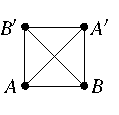
\includegraphics[width=\linewidth]{assets/ex28-network.pdf}
\end{minipage}
\end{exercise}

\begin{exercise}\label{ex:29}
证明，对每个具有非空内部且 $|\Omega|=1$ 的紧区域 $\Omega\subset\R^d$，以及每个 $\alpha<1-1/d$，都有 $d_\alpha(\mathscr L_\Omega,\delta_0)=+\infty$.
\end{exercise}

\begin{exercise}\label{ex:30}
考虑 $\alpha=1/2$ 时，两个原子测度 $\mu=\sum_i a_i\delta_{x_i}$ 与 $\nu=\sum_j b_j\delta_{y_j}$ 之间的分支运输. 考虑一个不属于任何 $x_i$ 或 $y_j$ 的点 $z$ 处的三岔结点：$z$ 处的三条分支，或者两条流入、一条流出，或者两条流出、一条流入. 证明，具有相同方向的两条分支必须构成 $90^\circ$ 角.
\end{exercise}
